\section{From movies to micrographs}
 \begin{figure}[H]
  \centering
  \captionsetup{width=.8\linewidth} 
  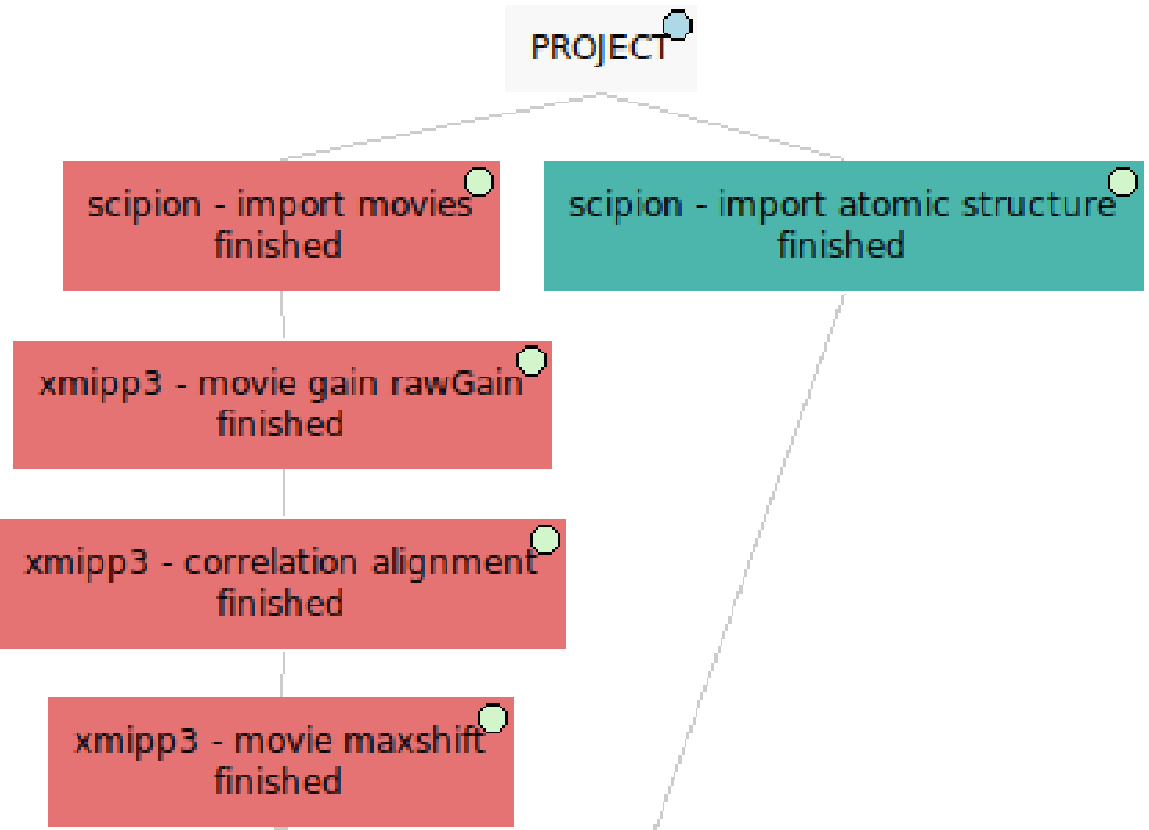
\includegraphics[width=0.65\textwidth]
  {{images/workflow_1.pdf}}
  \caption{From movies to micrographs workflow.}
  \label{fig:workflow_1}
  \end{figure}

 \subsection*{Import movies}
The protocol \scommand{scipion-import movies} allows to download the mouse apoferritin cryo-EM data in \scipion. The protocol form with parameters can be seen in \ffigure{fig:import_movies}. With this protocol, besides the set of movies, located in the Data folder, acquisition parameters such as accelerating voltage, spherical aberration and sample rate, will be registered in your \scipion project. 
 
 \begin{figure}[H]
  \centering
  \captionsetup{width=.8\linewidth} 
  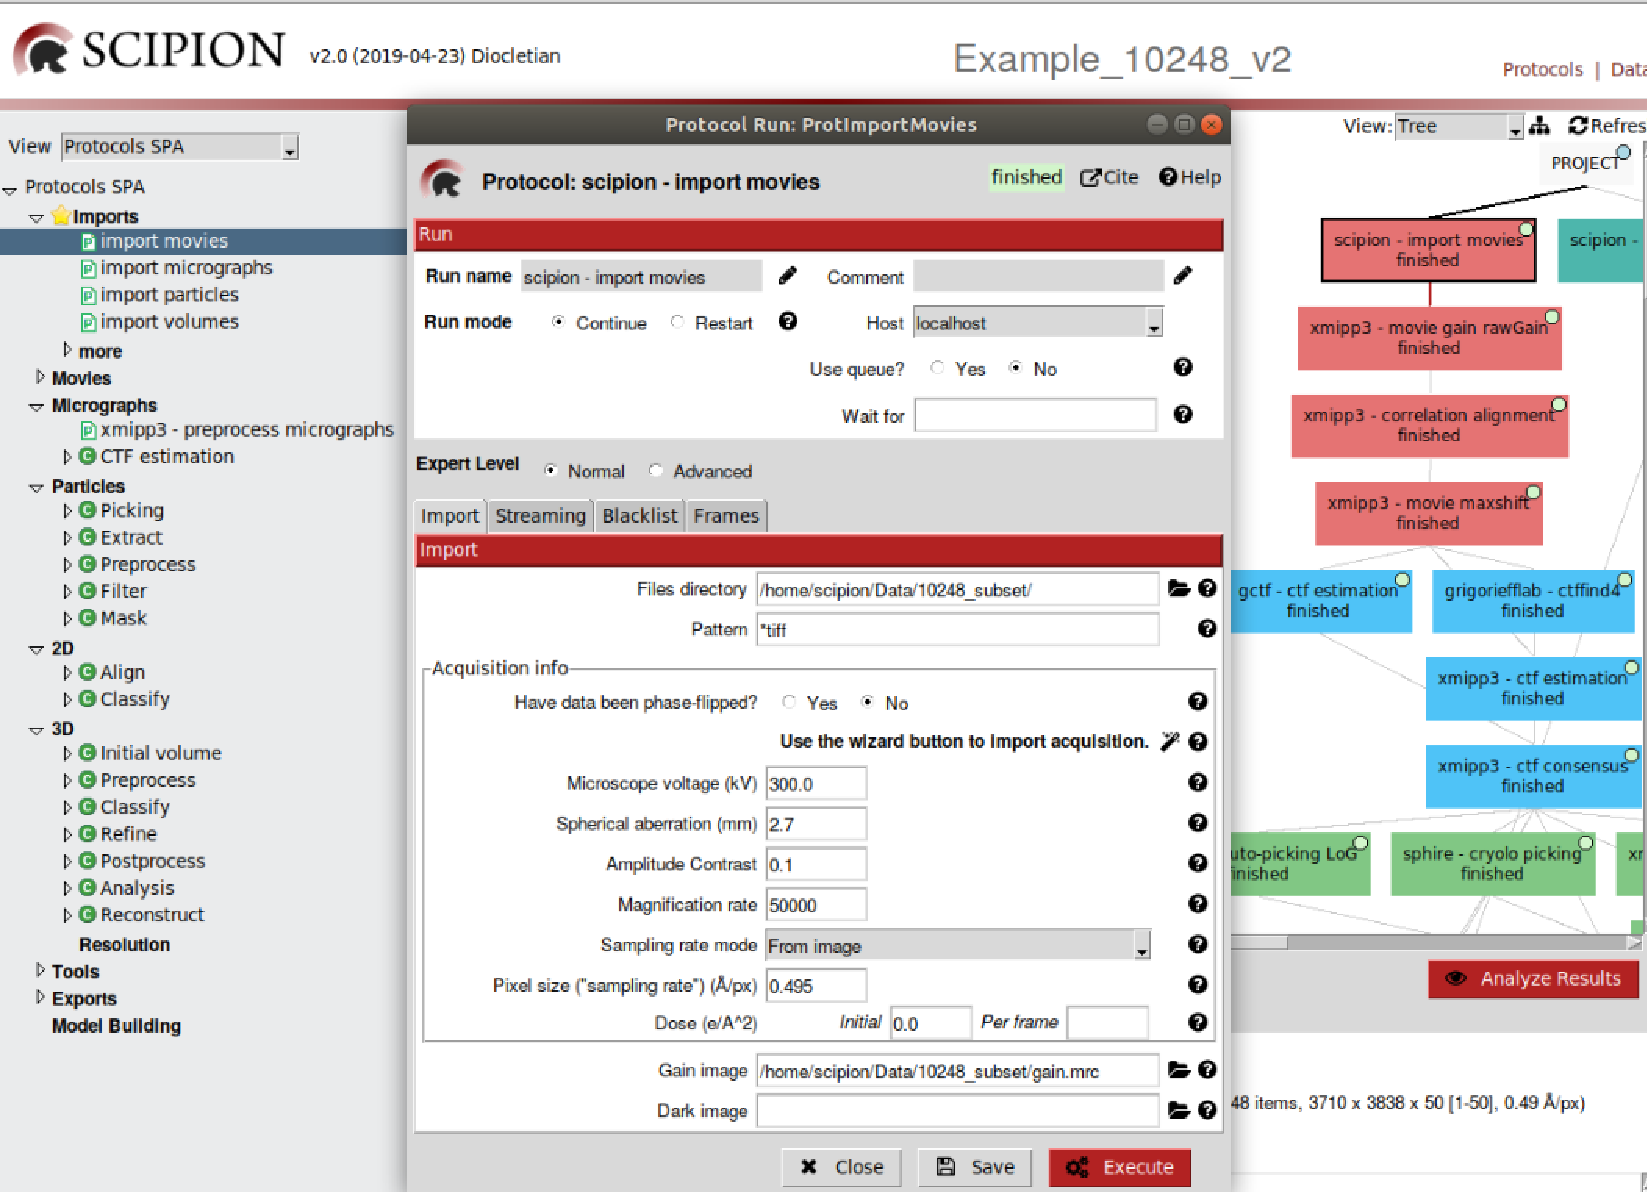
\includegraphics[width=0.95\textwidth]
  {{images/import_movies.pdf}}
  \caption{Filling in the protocol to import cryo-EM data.}
  \label{fig:import_movies}
  \end{figure}
  
After executing this protocol, we can visualize the list of 48 movies imported to the project by pressing \scommand{Analyze Results}. Each movie contains 50 frames with size 3710 pixels x 3838 pixels. Frames contained in each movie can be visualized by right-clicking each entry.
 
 \subsection*{Computation of movie gain}
 
The protocol \scommand{xmipp3-movie gain} is used to compute the movie gain (\ffigure{fig:movie_gain}). Two movie gains will be computed: 1) Without applying the input gain, to orientate the input movie gain; 2) Applying the input gain to estimate the residual movie gain.

\begin{figure}[H]
  \centering
  \captionsetup{width=.8\linewidth} 
  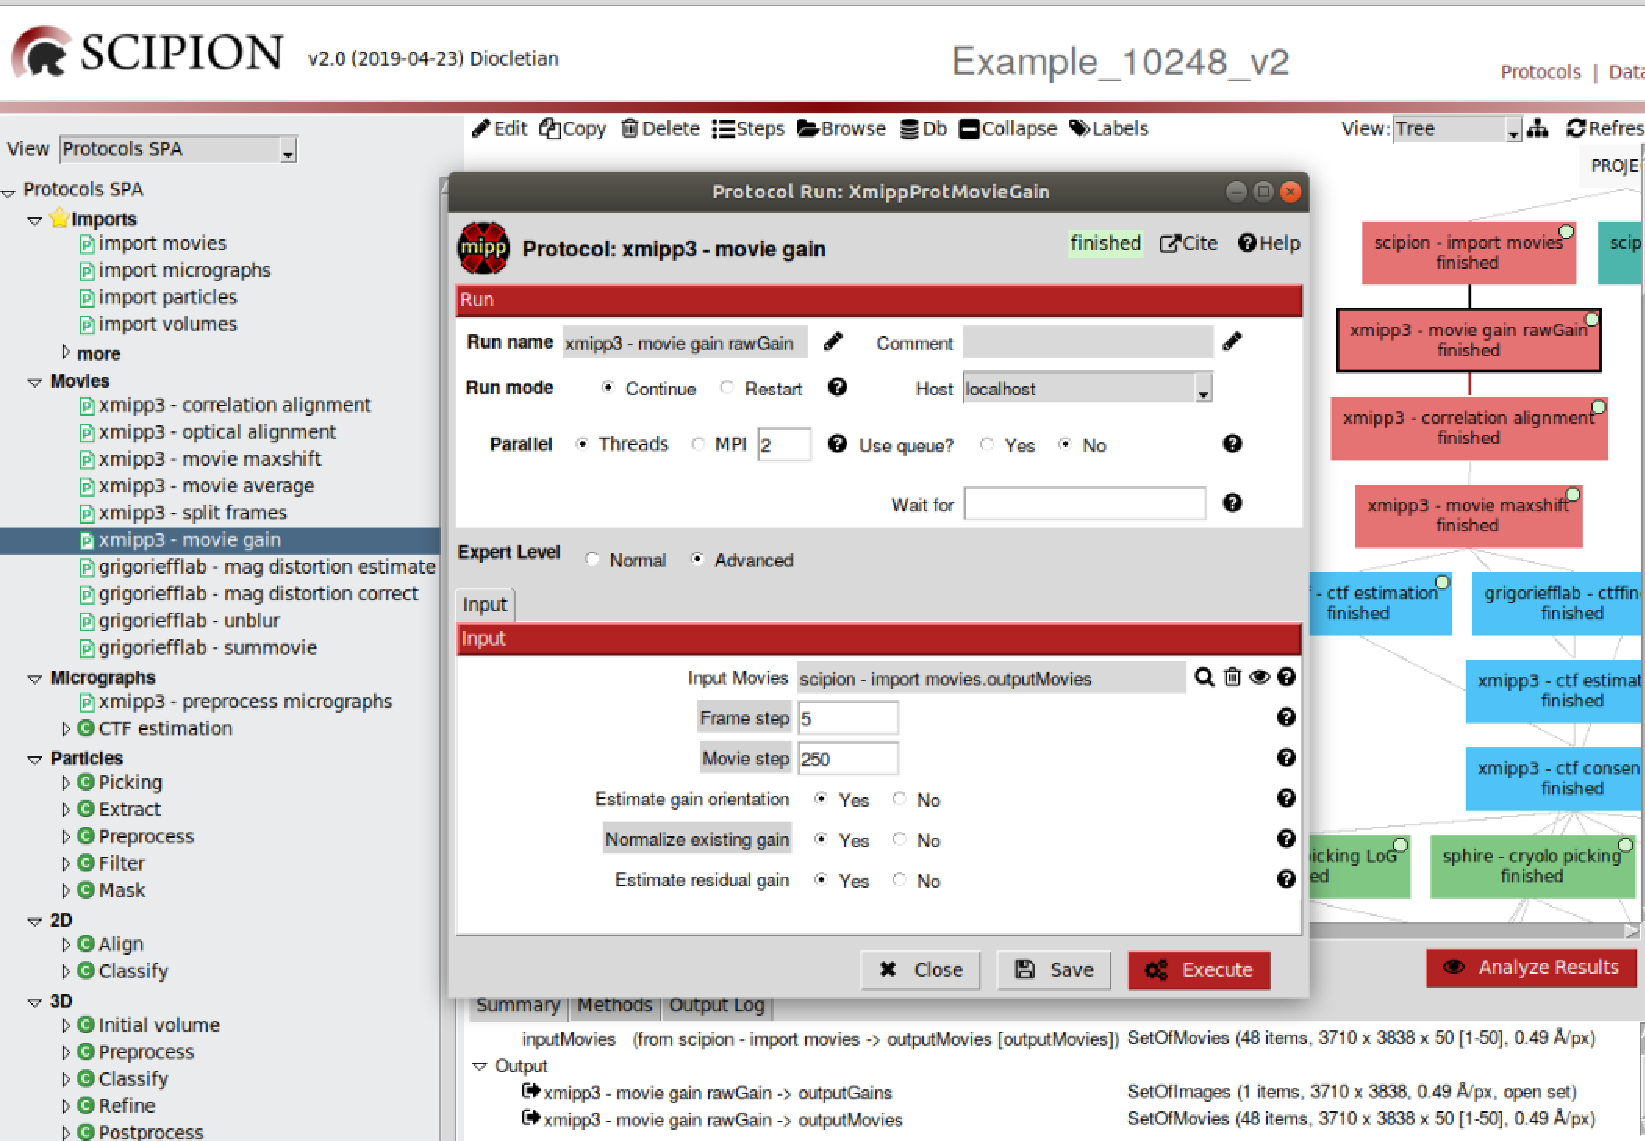
\includegraphics[width=0.95\textwidth]
  {{images/movie_gain.pdf}}
  \caption{Completing the protocol to compute the movie gain.}
  \label{fig:movie_gain}
  \end{figure}
 
After executing this protocol, by pressing \scommand{Analyze Results} we can visualize the image of the gain computed. None of the movie gains computed moves forward the protocol output.

 \subsection*{Movie alignment}
In order to correct BIM-induced image blurring and restore important high resolution information, the stack of individual frames contained in each movie needs to be aligned. Only one image will be generated, and this image is called micrograph. Although in \scipion we have integrated several protocols to perform global and local alignment, in this tutorial we are going to use \scommand{xmipp3-correlation alignment}. We have completed the params of this protocol in \ffigure{fig:correlation_alignment}.

\begin{figure}[H]
  \centering
  \captionsetup{width=.8\linewidth} 
  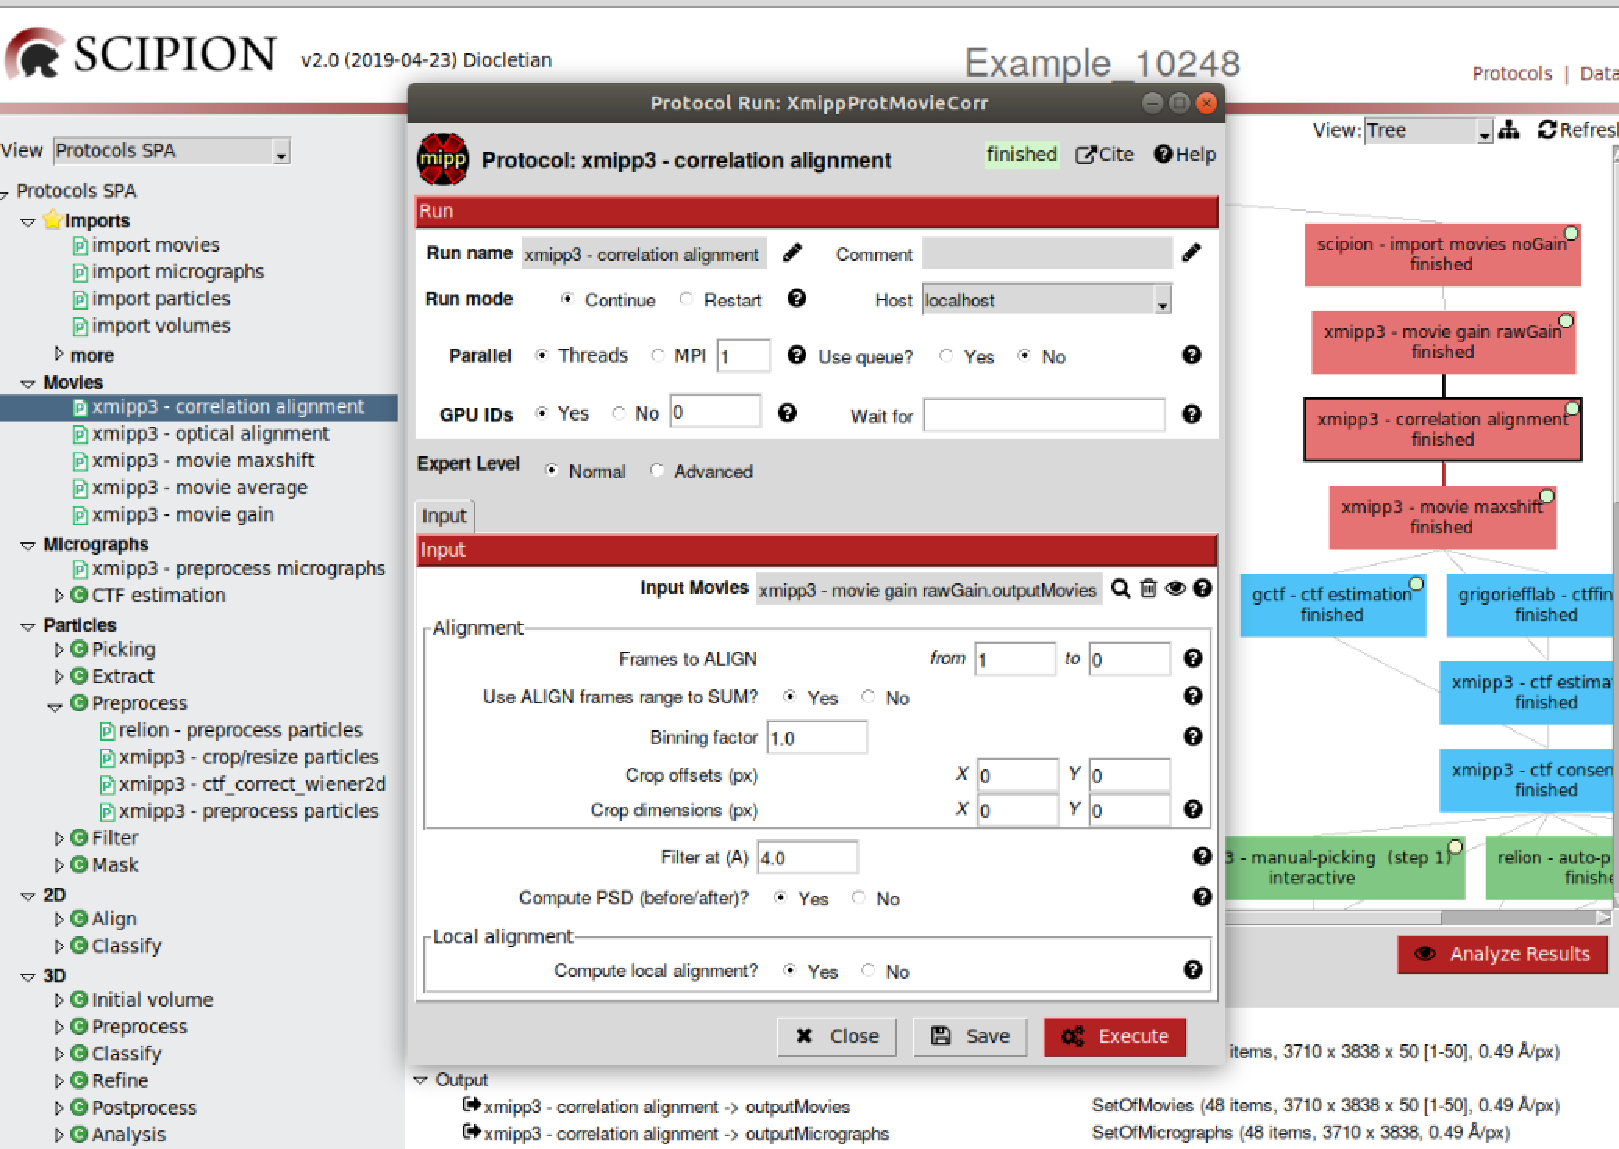
\includegraphics[width=0.95\textwidth]
  {{images/correlation_alignment.pdf}}
  \caption{Filling in the protocol to align the frames of each movie.}
  \label{fig:correlation_alignment}
  \end{figure}
  
When the execution of this protocol finishes, we can observe the list of the set of 48 resulting micrographs by pressing \scommand{Analyze Results}. The first column contains composite images with half of the PSD of the unaligned micrograph (left side) and half of the PSD of the aligned one (right side). The plots in the second column reflect accumulated shifts of the movie frames. The name of each resulting micrograph appears in the third column. Each micrograph included in the set generated can be opened for visual inspection by right-clicking its entry. 

\subsection*{Screening of micrographs}

Since some of the micrographs generated in the previous step could derive from movies with high drift among frames, we have added in the processing workflow a step to select only the micrographs originated from movies with allowed drifting values among frames. The protocol \scommand{xmipp3-movie maxshift}, completed in \ffigure{fig:movie_maxshift}, was designed to screen micrographs according maximum shift values. Movies will be rejected if they exceed the maximum shift value among frames, the maximum travel value for the whole movie, or both previous conditions.

\begin{figure}[H]
  \centering
  \captionsetup{width=.8\linewidth} 
  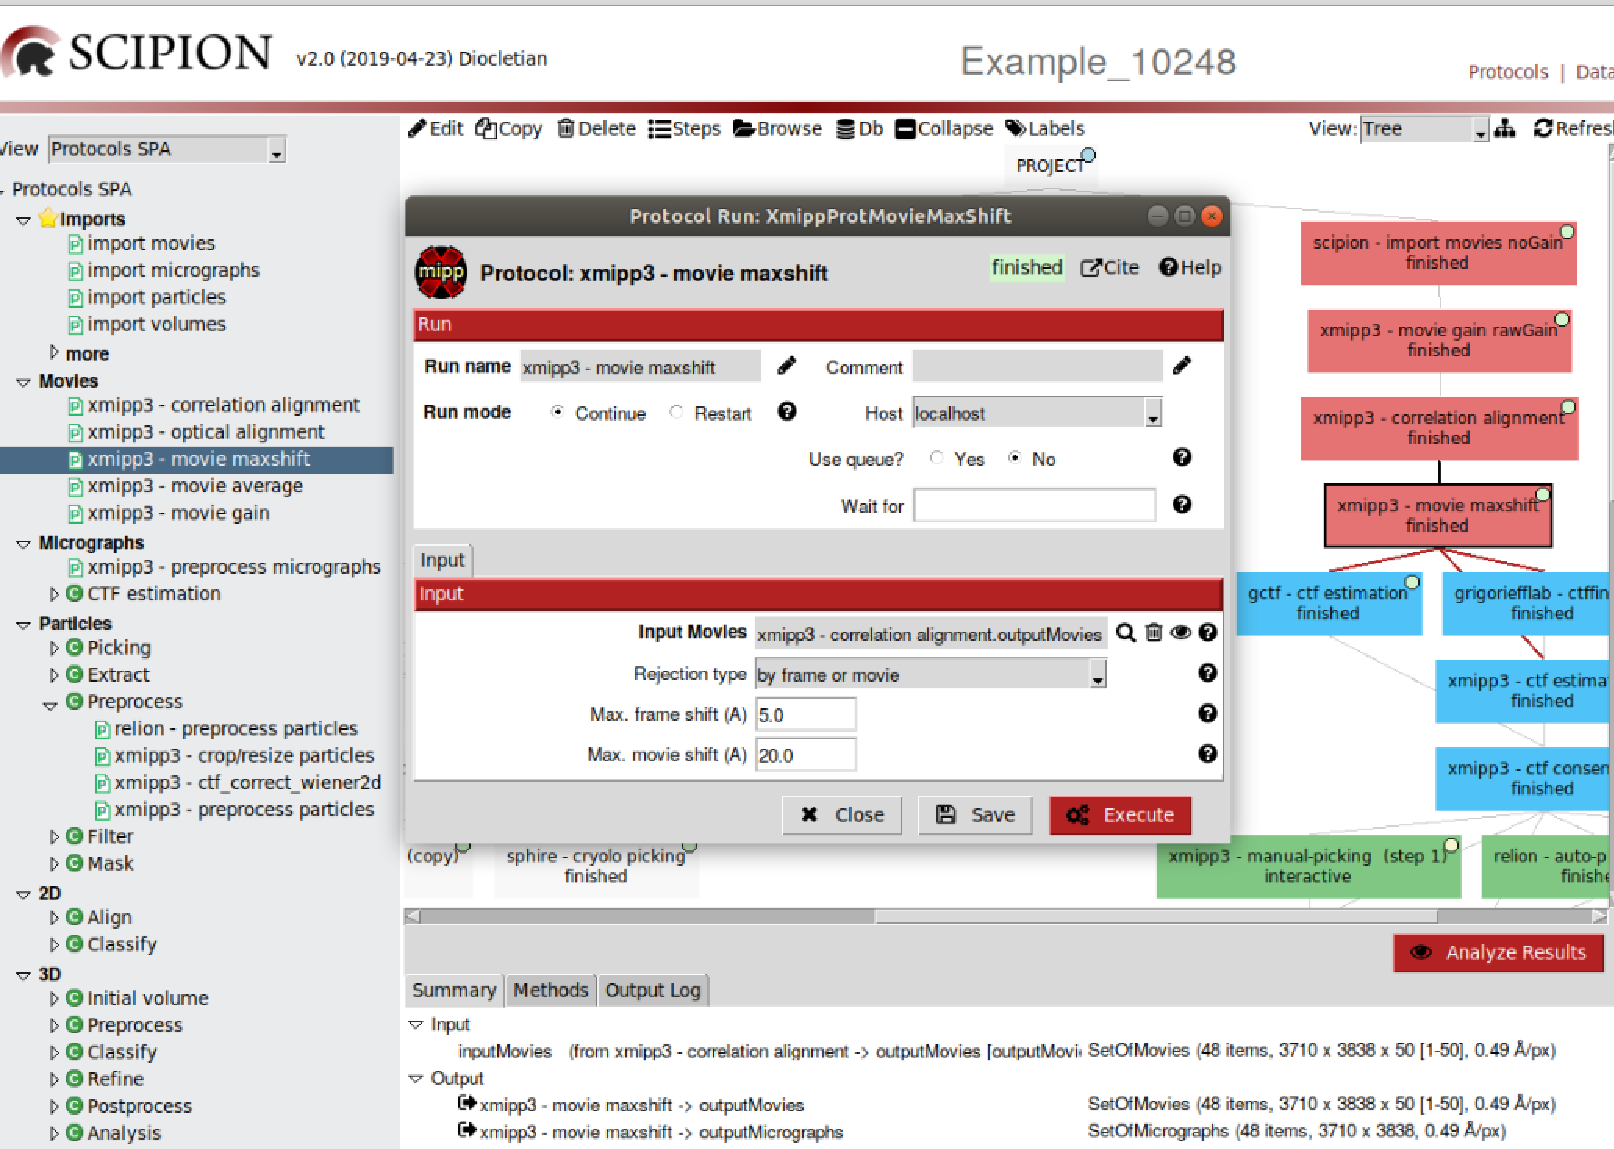
\includegraphics[width=0.95\textwidth]
  {{images/movie_maxshift.pdf}}
  \caption{Completing the protocol to screen the micrographs.}
  \label{fig:movie_maxshift}
  \end{figure}
  
  Once the protocol is executed, both discarded and accepted lists of micrographs can be visualized by pressing \scommand{Analyze Results}. Each micrograph can be opened for visual inspection by right-clicking. In this case, the set of 48 input micrographs have been included in the protocol output. This set will serve as input for further processing steps.
